\documentclass[11pt,a4paper]{amsart}

% Include AMS packages
\usepackage{amsmath,amsthm,amssymb}
\usepackage{tikz}
\usepackage{listings}
\lstset{breaklines=true, language=Python, basicstyle=\footnotesize, showstringspaces=false}


% Include graphics packages, if necessary:
% delete the %-sign in front of the 
% relevant \usepackage command.

% graphicx for including image files
%\usepackage{graphicx}

% pgfplots, for plotting graphs
%\usepackage{pgfplots}

% Change paragraphs from indented to line spaces
% (Remove or comment out if not needed)
\usepackage{parskip}

% Set up theorems, propositions etc
\newtheorem{thm}{Theorem}[section]

\theoremstyle{plain}
\newtheorem{prop}[thm]{Proposition}
\newtheorem{lem}[thm]{Lemma}

\theoremstyle{definition}
\newtheorem{defn}[thm]{Definition}

\theoremstyle{remark}
\newtheorem{rem}[thm]{Remark}
\newtheorem{note}[thm]{Note}
\newtheorem{eg}[thm]{Example}
\newtheorem{egs}[thm]{Examples}

% Include title, author and date, as appropriate
\title{MAS115: Semester 1 Mini-project}
\author{180188428}
\date{$5^{\text{th}}$ November}
\begin{document}
\maketitle

\section{Theory}

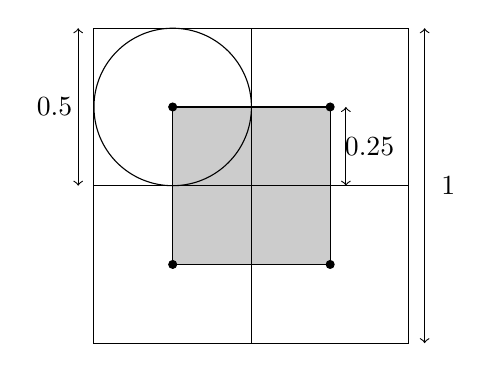
\begin{tikzpicture}
	\filldraw[fill=black!20] (-1,-1) rectangle (1,1);
	\draw (-2,0) -- (2,0);
	\draw (0,2) -- (0,-2);
	\draw (-2,-2) rectangle (2,2);
	\draw (-1,1) circle (1);
	\draw[<->] (1.2,0) -- (1.2, 1);
	\draw[<->] (2.2, 2) -- (2.2, -2);
	\node at (1.5, 0.5) {\Small 0.25};
	\node at (2.5, 0) {1};
	\draw[<->] (-2.2,0) -- (-2.2, 2);
	\node at (-2.5, 1) {0.5};
	\filldraw[fill=black] (1,1) circle (0.05);
	\filldraw[fill=black] (1,-1) circle (0.05);
	\filldraw[fill=black] (-1,1) circle (0.05);
	\filldraw[fill=black] (-1,-1) circle (0.05);
	
\end{tikzpicture}

The way I started this project off, was by visualising where the centre of the disk can lie within one square on the chess board whereby it is only covering one colour. I did this by drawing the diagram above which represents one square on the chess board split into quadrants with the disk inside one. The shaded region shows the area of the square where the centre of the disk can land so that it only covers the one square and doesn't touch another colour. In my interpretation of this project, I am including the green table as an extra colour so if the disk is half on the chess board and half on the green table then it is covering more than one colour.

Each corner of the shaded square is the centre of each quadrant of the square of length one. This gives the shaded square an area of $0.5{units}^2$. So, multiplying this area by the number of squares on the chess board gives the total area on the board where the disk can land and only cover one colour. $0.5{units}^2(64) = 16units^2$. Using this value to calculate the proportion of the board that is shaded, we get $\frac{16}{64}=\frac{1}{4}$. This shows us that the disk can land in a quarter of the board and only be covering one colour. But how do we know that a random point where the disk drops, lands in the shaded region?

\section{Analysing code}

I have modelled the chess board as a Cartesian $xy$ plane where the bottom left corner of the chess board is at $(0, 0)$ and the top right is at the point $(8, 8)$. I have chosen to have 801x801 points in the chess board for when random points are chosen (from 0 to 800). The code for choosing these random points is below. 
\begin{lstlisting}
for i in range(number_of_disk_drops):
    x_r= random.randint(0, 800)/100
    y_r= random.randint(0, 800)/100
    print("Random point: (",x_r,",", y_r,")")
\end{lstlisting}
The shaded region of a square is within $+0.25$ and $+0.75$ of the integer value $x$ and $y$ coordinate. So we need an "if" statement with some inequalities to determine whether the random point is in the shaded region.
\begin{lstlisting}
    if 0.25 <= x_r - int(x_r) <= 0.75:
        if 0.25 <= y_r - int(y_r) <= 0.75:
            one_colour = one_colour + 1
\end{lstlisting}
If the $x$ and the $y$ coordinate of the random point is within the shaded region then the variable, \begin{verbatim} one_colour \end{verbatim} will be increased by one.

\subsection{Outputs}

I have a few outputs in my code to give more clarity on how things are calculated. The first, is printing how many instances there are of the disk covering only one colour and the other two are the proportions of the disk drops that have covered either one colour or more than one colour.

\begin{lstlisting}
print("One colour covered", one_colour, "times")

print("Proportion that only one colour is covered = ", one_colour/number_of_disk_drops)

print("Proportion that more than one colour covered = ", 1 - (one_colour/number_of_disk_drops))
\end{lstlisting}

From these proportions, I can calculate the probability of the disk covering one colour and more than one colour. Using the law of large numbers which states that when the frequency of a trial is high, the proportion of the outcomes will tend to their theoretical probability. Looking at one square of the chess board as a Cartesian $xy$ plane with 101x101 points (0 to 100), there are 51 $x$ coordinates and 51 $y$ coordinates (25 up to 75) where the disk can drop and be covering one colour. The probability of the disk landing in this area is $\frac{51^2}{101^2}$ which is approximately 0.255. Subtracting this from 1 gives the probability of the disk covering more than one colour which is approximately 0.745.

Geometrically, the probability of the disk landing in the shaded region is a quarter because the area of the shaded region of one square on the chess board is a quarter of the whole square. However, computationally, because we have included both +0.25 and +0.75 in our inequalities to determine where the disk can drop, this gives slightly more than a quarter of the square because both extremities are included. If 0.25 or 0.75 was not included in the inequalities, then the probability will tend to a quarter.

\section{Varying the size of the disk}
If the diameter of the disk was bigger, then the probability of the disk landing on the chess board covering more than one colour will be higher. This is because if the diameter is bigger, then the disk's area will also be bigger so it has a much smaller chance of it landing within one square. If the diameter of the disk was changed to be greater than one, then there will be zero chance of the disk covering only one colour. For example, if the diameter of the disk was changed from 0.5 to 0.75 then the code for determining whether the disk in these random points is covering one colour would be changed to:
\begin{lstlisting}
    if 0.375 <= x_r - int(x_r) <= 0.625:
        if 0.375 <= y_r - int(y_r) <= 0.625:
            one_colour = one_colour + 1
\end{lstlisting}
Here, I have changed the boundaries on the inequalities from 0.25 and 0.75 to 0.375 and 0.625. This has reduced the area of the shaded region in which the centre of the disk can land.

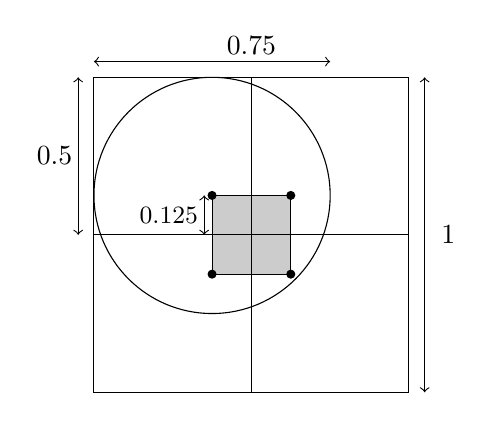
\begin{tikzpicture}
	\filldraw[fill=black!20] (-0.5,-0.5) rectangle (0.5,0.5);
	\draw (-2,0) -- (2,0);
	\draw (0,2) -- (0,-2);
	\draw (-2,-2) rectangle (2,2);
	\draw[<->] (2.2, 2) -- (2.2, -2);
	\node at (2.5, 0) {1};
	\draw[<->] (-2.2,0) -- (-2.2, 2);
	\node at (-2.5, 1) {0.5};
	\draw(-0.5,-0.5) rectangle (0.5,0.5);
	\draw[<->] (-0.6,0.5) -- (-0.6,0);
	\node at (-1.05,0.25) {\small0.125};
	\draw(-0.5,0.5) circle (1.5);
	\draw[<->] (-2,2.2) -- (1,2.2);
	\node at (0,2.4) {0.75};
	\filldraw [fill=black] (-0.5,0.5) circle (0.05);
	\filldraw [fill=black] (-0.5,-0.5) circle (0.05);
	\filldraw [fill=black] (0.5,0.5) circle (0.05);
	\filldraw [fill=black] (0.5,-0.5) circle (0.05);
\end{tikzpicture}

 For simplicity I have modelled this as a Catesian $xy$ plane with 1001x1001 points to avoid decimals. The probability of the disk landing in this shaded region is $\frac{251^2}{1001^2}$ since there are 251 $x$ and $y$ coordinates (from 375 to 625) where the disk can land. This probability is approximately 0.0629, giving the probability of the disk covering more than one colour to be approximately 0.937.




\end{document} 